\chapter{FUNDAMENTAÇÃO TEÓRICA} \label{cap:funda}

Nessa seção será descrito o estado da arte do tema escolhido. Primeiramente será dado uma breve introdução sobre processamento de imagem, dando maior ênfase no processo de análise de imagem, seguindo teoria de Gonzales e Woods. Este capítulo também será utilizado para descrever o funcionamento de um sistema OCR.

\section{Processamento Digital de Imagens}

O objeto de operação do Processamento Digital de Imagens são as imagens digitais\cite{Almeida2018}. Uma imagem na forma digital é representada através de matrizes, as quais mapeiam as cores reais da imagem, do mundo físico para o digital.



A área de PDI vem evoluindo constantemente no decorrer dos anos, com uma ampliação significativa dos estudos envolvendo morfologia matemática, redes neurais, processamento de imagens coloridas, compressão de imagens, reconhecimento de imagens e sistemas de análise de imagens baseados em conhecimento \cite{GONZALEZ2002}. 

Os sistemas de PDI consistem em um conjunto de técnicas que possibilitam a captura de imagens por meio de equipamentos variados, como tomógrafos médicos, câmeras fotográficas, satélites e outros, tal como a representação e transformação destas imagens. O propósito é fazer a extração e identificação das informações que fazem parte das imagens, de forma automática por meio de máquinas \cite{PEDRINI2008}. Nas próximas seções está descrito alguns conceitos empregados em PDI, bem como técnicas voltadas para o reconhecimento e interpretação de padrões, úteis na composição de sistemas desta natureza. 


\subsection{Representação de Imagens Digitais}

Uma imagem pode ser representada no plano cartesiano por uma função f(x,y), onde x e y são coordenadas espaciais. A função f(x,y) possui, comumente, um valor em níveis de cinza, ou cor, em qualquer ponto da imagem, o ponto de origem representado pela coordenada (0,0) fica situado no canto superior esquerdo da imagem \cite{Goncalves2016}.

A Figura 1 ilustra como seria um imagem digital em forma de notação matricial. Os elementos dessa matriz são chamados de elementos pictóricos, elementos de imagens, pels e pixel. O \textit{Pixel} (contração de Picture element) é o termo mais utilizado \cite{GONZALEZ2006}. O índice m representa a linha na qual o pixel se encontra, enquanto que o índice n aponta a coluna na qual está localizado o pixel. Em uma imagem M linhas e N colunas, m terá seu valor variando de 0 até M-1 e n terá seu valor variando de 0 até N-1. Em uma representação de imagens monocromáticas em que os tons de cinza representam o brilho da imagem, a representação da matriz tem seus valores variando de 0 a 255, preto ao branco respectivamente \cite{Almeida2018}. 

 \begin{figure}[htb]
	\centering
	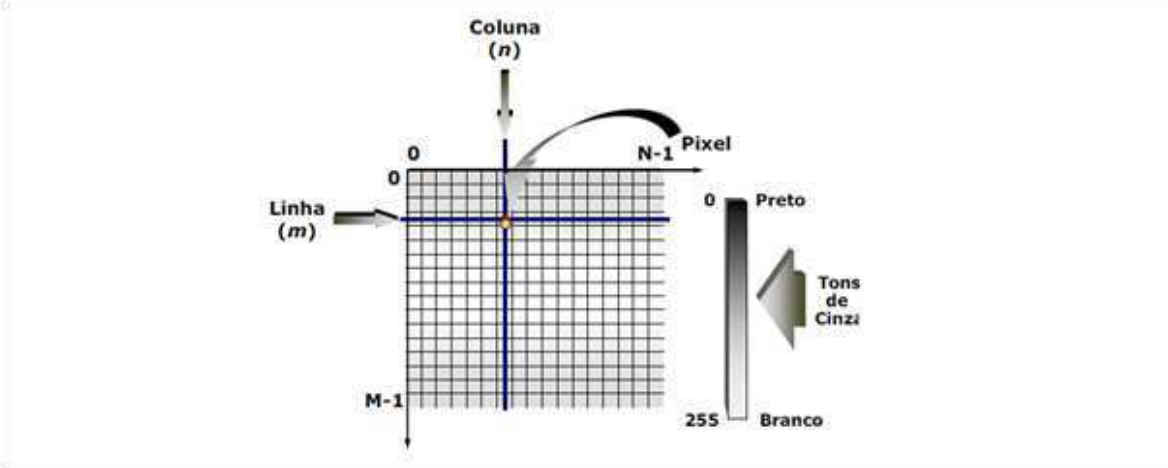
\includegraphics[width=1.0\textwidth]{Imagens/imagem1} 
	\caption[Texto que vai aparecer na lista de fig.]{Representação da imagem em uma matriz bidimensional.}
\fonte{\citeonline{Goncalves2016}}
	\label{fig:tux_laplace}
\end{figure}


\subsection{Vizinhança e Conectividade}
Em uma imagem digital existem vários relacionamentos importantes entre os pixels. Conforme descrito em \citeonline{GONZALEZ2002}, 
um pixel p de coordenadas (x,y) possui uma vizinhança horizontal e vertical determinadas por (x-1, y), (x+1, y) e (x, y-1), (x, y+1) denominada vizinhança-4, e também uma vizinhança diagonal composta pelas coordenadas (x-1, y-1), (x-1, y+1), (x+1, y-1) e (x+1, y+1). Convencionado com o nome de vizinhança-8, a união destas vizinhanças.

Deve-se levar em consideração que nos pixels das extremidades da imagem, terão vizinhos faltantes. Demonstrado visivelmente na Figura 2, o conceito de vizinhança de um pixel.

A conectividade entre pixels é um conceito importante no processamento de imagens, em especial para o reconhecimento de bordas de objetos presentes em uma imagem. Para identificar se dois pixels são conexos, é preciso averiguar se são vizinhos e se seus níveis de cinza são similares \citeonline{Goncalves2016}. É fundamental analisar a possibilidade de haver conexidade por meio da utilização da vizinhança-4 ou utilizando a vizinhança-8.

 \begin{figure}[htb]
	\centering
	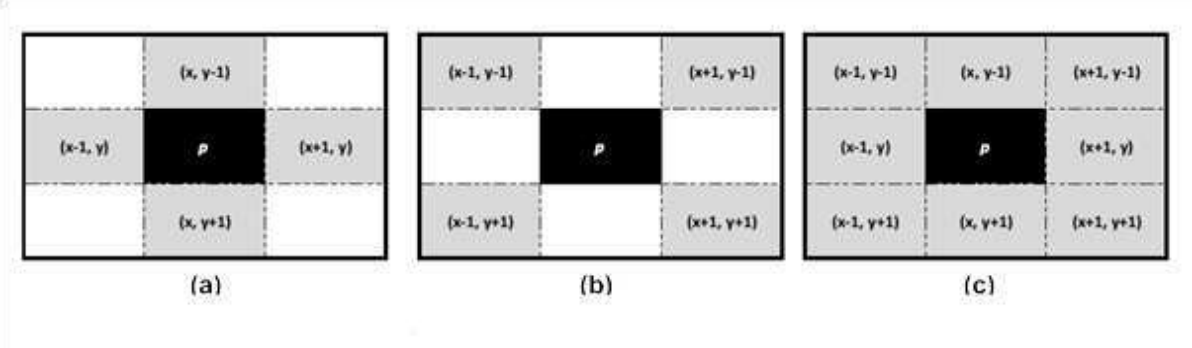
\includegraphics[width=1.0\textwidth]{Imagens/imagem3} % <- formatos PNG, JPG e PDF
	\caption[Texto que vai aparecer na lista de fig.]{Tipos de vizinhança. (a) Vizinhança-4; (b) Vizinhança diagonal; (c) Vizinhança-8.  (a) Imagem; (b) Histograma.}
\fonte{\citeonline{Goncalves2016}}%citaç\~ao do livro onde pegou a figura	
	\label{fig:tux_laplace}
\end{figure}



\section{Ciclo de Gonzalez}
(PEDRO: atualizar imagem conforme livro de 2018)
Segundo \citeonline{GONZALEZ1992}, as técnicas em análise de imagem podem ser divididas em três áreas básicas: (1) aquisição e processamento de baixo nível, com funções que podem ser vistas como reações automáticas, ou seja, reações que não requerem comportamento inteligente; (2) processamento de nível intermediário, com processos de extração e caracter- ização de componentes em uma imagem; e (3) processamento de alto nível, que envolve os processos de reconhecimento e interpretação. A Figura 3 mostra os processos de cada uma dessas áreas.

 \begin{figure}[htb]
	\centering
	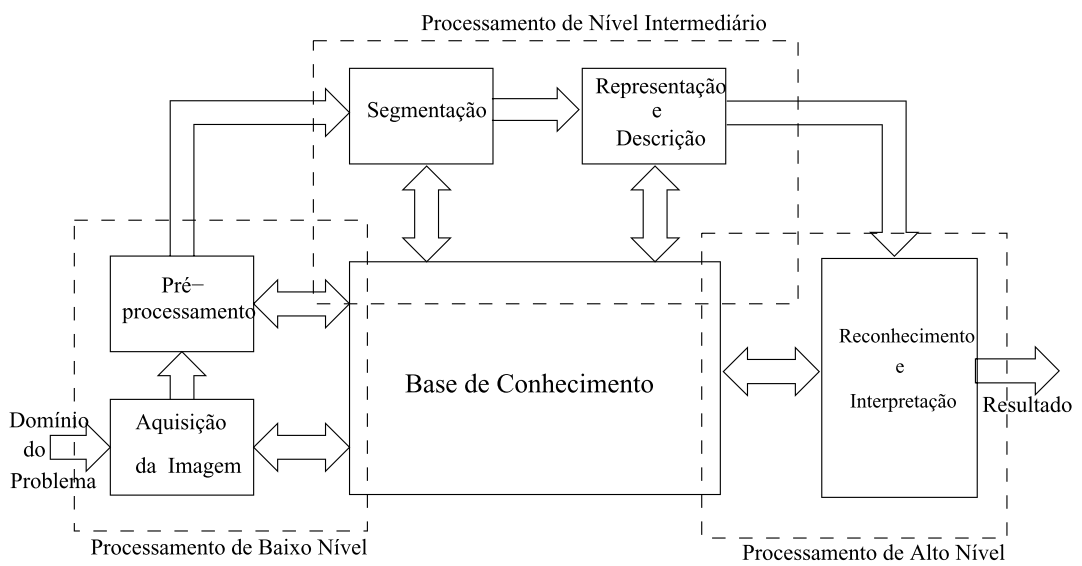
\includegraphics[width=1.0\textwidth]{Imagens/imagem5} % <- formatos PNG, JPG e PDF
	\caption[Elementos do processo de análise de imagem.]{Elementos do proceso de análise da imagem. }
\fonte{\citeonline{GONZALEZ1992}}%citaç\~ao do livro onde pegou a figura	
	\label{fig:tux_laplace}
\end{figure}

Nas seções 2.2.1 a 2.2.6 serão apresentado os passos para o processamento digital de imagens com enfoque em pré-processamento de imagens, são eles:
\begin{itemize}
\item Aquisição de imagem;
\item Pré-processamento;
\item Segmentação;
\item Representação e descrição;
\item Reconhecimento;
\item Interpretação.
\end{itemize}

\subsection{Aquisição de imagem}
O primeiro passo do processo de reconhecimento é a aquisição da imagem. Segundo \citeonline{GONZALEZ1992}, o primeiro passo do processo requer apenas um sensor de imagens e a capacidade para digitalizar o sinal produzido pelo
sensor

São necessários dois elementos para a aquisição da imagem: um aparelho físico que é sensível à faixa espectral de energia eletromagnética. Um exemplo de dispositivo bastante utilizado para este fim é a câmera Charge Coupled Device (\sigla{CCD}{Charge Coupled Device}) que hoje comumente vem acoplado em todos os smartphones do mercado, com capacidades que podem chegar a Ultra HD (3840x2160 pixels). E um digitalizador, que converte o sinal elétrico capturado na sua forma digital.


\subsection{Pré-processamento}
Após a aquisição e digitalização da imagem, o próximo passo é o pré-processamento. A função chave do pré-processamento é melhorar a imagem, com o objetivo de aumentar as chances de sucesso dos processos seguintes \cite{GONZALEZ1992}. Nesta etapa, são utilizadas técnicas para aumento de contraste, remoção de ruídos, realce, normalização etc., com o objetivo de converter os padrões para uma forma que possibilite uma simplificação do posterior processo de reconhecimento \cite{Rodrigues2002}.

\subsection{Segmentação}

O próximo estágio é o processo chamado de segmentação, a segmentação de imagens consiste em dividir uma imagem de entrada em partes
constituintes, para uma melhor caracterização das regiões de interesse (\sigla{ROI}{Região de Interesse}). As operações de segmentação procuram isolar regiões de pontos da imagem pertencentes a objetos, para
posterior extração de atributos \cite{Lourdes2010}.

De um modo geral, as técnicas de segmentação utilizam duas abordagens
principais: a similaridade entre os pixels e a descontinuidade entre eles. A binarização de imagens, técnica baseada em similaridade, é a técnica mais utilizada, é uma  simples e eficiente técnica do ponto de vista computacional, sendo portanto comumente utilizada em sistemas de visão computacional \cite{ISRAEL2003}.


Na segmentação com descontinuidade entre os pixels, a segmentação é baseada nas técnicas de limiarização, crescimento por regiões, união e divisão de regiões \cite{Rodrigues2002}.


\subsection{Representação e Descrição}

Normalmente, após a segmentação, dados brutos de pixel são obtidos. Por consequência, pode ser fundamental o processo de converter os dados para uma forma apropiada, possibilitando o processamento digital. 

Dois tipos de representação podem ser utilizados: representação limite ou representação regional. Quando o foco está com características de localização nas extremidades, como por exemplo cantos e bordas da imagem, é apropriada a representação limite. Representação regional é apropriada quando o foco está localizada no centro da imagem e é possível encontrar uma vizinhança-8. Escolher a representação é apenas uma parcela da solução para a conversão de dados brutos em uma forma adequada para o processamento computacional. \cite{Rodrigues2002}


Segundo \citeonline{GONZALEZ1992}, deve ser utilizado como complemento, um método para descrever os dados tal que as características de interesse sejam realçadas. Descrição, também chamada de seleção de característica, lida com a extração de características que resultam em algumas informações quantitativas de interesse ou que são básicas para diferenciar uma classe de objetos de outra.

\subsection{Reconhecimento}
O ultimo estágio no processo de análise da imagem envolve reconhecimento e interpretação. Reconhecimento é o processo que fixa um rótulo a um objeto baseado na informação fornecida pelos seus descritores. Interpretação envolve a fixação de significado a um grupo de objetos reconhecidos. Para resolver problemas de reconhecimento pode-se partir de três abordagens: estatística, estrutura e neural. Nesta dissertação, o problema de reconhecimento da imagem é tratado com detecção de bordas e ajuste de perspectiva, preparando a imagem para ser utilizada por um sistema de reconhecimento de caracteres, assuntos que serão abordados nas próximas sessão \cite{GONZALEZ1992}.



\section{Detecção de Bordas}

Uma borda é definida por uma mudança repentina do nível de cinza, ou seja ocorre uma descontinuidade no tom de cinza. Dessa forma, a descontinuidade pode ser percebida quando o gradiente da imagem tem uma brusca variação \cite{Antonio}. 

Em linhas gerais, para determinar se um pixel da imagem é ou não de borda, calcula-se o gradiente deste pixel e, caso o gradiente seja maior do que um valor de limiar pré-definido, o pixel é considerado como borda \cite{Silva2001}.

A detecção de bordas é essencial na presente dissertação para encontrar o objeto em destaque da imagem de entrada e pode ser feito com métodos de pré-processamento. Uma aplicação de filtro mediana, para reduzir os ruídos e em seguida um filtro passa-altas, para realce nos contornos
ou bordas dos objetos na imagem \cite{ISRAEL2003}. 

Neste trabalho o escaneamento de bordas foi baseado  através de bulas e caixas de remédios, que basicamente possuem uma forma retangular e por ser um retangulo, o mesmo possui quatro arestas. Portando, é possível criar uma simples heurística para ajudar a criar um contorno de bordas no foco da imagem. 

Com a analise de bordas concluída, o resultado obtido é a ROI, que representa a região considerada importante da imagem.




\section{Correção de Perspectiva}

//todo estudos nao finalizados. tópico importante
//iPhone and Android “scanner” apps that let you snap a photo of a document and then have it “scanned” into your phone
//four_point_transform


